\documentclass[aspectratio=169,11pt]{beamer}
\usetheme{Madrid}
\usecolortheme{default}
\setbeamertemplate{navigation symbols}{}
\usepackage{booktabs}
\usepackage{array}

\title[Process Monitor \& Job Scheduler]{CPU / Process Monitor and Job Scheduler}
\subtitle{Software Systems Lab Project}
\author[Rahul, Ganesh]{Rahul Ahirwar (CS25BT011) \and Ganesh (CS25BT010)}

\begin{document}

% ---------------------------------------------------------------
% 1. Topic, team and roles (one page)
\begin{frame}
  \centering
  \begin{beamercolorbox}[sep=10pt,center,rounded=true,shadow=true]{title}
    {\Large CPU / Process Monitor and Job Scheduler}\\[3pt]
    {\small Software Systems Lab Project \textbullet{} IIT Dharwad \textbullet{} November 2026}
  \end{beamercolorbox}
  \vspace{0.5cm}

  \begin{tabular}{p{0.22\textwidth}p{0.62\textwidth}}
    \toprule
    \textbf{Member} & \textbf{Role} \\
    \midrule
    \textbf{Rahul Ahirwar}\newline CS25BT011 &
      Design and all the code: scheduling algorithms and statistics,
      process monitor and tree, real process scheduler (threads, signals),
      Tkinter GUI and plots, bash scripts, tests, profiling, Git \\[6pt]
    \textbf{Ganesh}\newline CS25BT010 &
      \LaTeX{} report, Beamer slides and the presentation \\
    \bottomrule
  \end{tabular}
  \vspace{0.4cm}

  \small \textbf{Course topics used:} Unix process hierarchy, process monitoring, threads,
  Python, GUI, plotting, bash, profiling, Git, \LaTeX
\end{frame}

% ---------------------------------------------------------------
% 2. Problem statement
\begin{frame}{Problem statement}
  \begin{itemize}
    \item A computer runs hundreds of processes, but one CPU core runs only one at a time.
    \item Two questions every operating system must answer:
      \begin{enumerate}
        \item \textbf{What is running now?} \(\rightarrow\) process monitoring
        \item \textbf{Who runs next?} \(\rightarrow\) CPU scheduling
      \end{enumerate}
  \end{itemize}
  \vspace{0.3cm}
  \begin{block}{Goal}
    Build an application that \textbf{tracks processes} and \textbf{schedules jobs}
    with FIFO, Priority and Round Robin, with status views and performance statistics.
  \end{block}
\end{frame}

% ---------------------------------------------------------------
% 3. Proposed approach
\begin{frame}{Proposed approach: how we solve the problem}
  \centering
  \begin{tabular}{>{\raggedright\arraybackslash}p{0.27\textwidth}>{\raggedright\arraybackslash}p{0.66\textwidth}}
    \toprule
    \textbf{Problem} & \textbf{How we solve it} \\
    \midrule
    \textbf{What is running now?} &
      Every 1.5\,s we read all running programs and show them in a table,
      a family tree and graphs. \\ \addlinespace[7pt]
    \textbf{Who runs next?} &
      We coded FIFO, Priority and Round Robin, drew a timeline for each
      and measured the waiting time. \\ \addlinespace[7pt]
    \textbf{Does it work for real?} &
      We run real programs and pause or resume them in turns. \\ \addlinespace[7pt]
    \textbf{Keep the app smooth} &
      Background threads collect data, so the app never freezes. \\ \addlinespace[7pt]
    \textbf{Is it fast and correct?} &
      We profiled to find the slow part (made it up to 133\(\times\) faster)
      and wrote 26 tests that all pass. \\
    \bottomrule
  \end{tabular}
  \vspace{0.4cm}

  \textbf{Steps:} read processes \(\rightarrow\) show them \(\rightarrow\)
  schedule jobs \(\rightarrow\) measure and test
\end{frame}

% ---------------------------------------------------------------
% 4. Results
\begin{frame}{Results}
  \begin{columns}[c]
    \begin{column}{0.55\textwidth}
      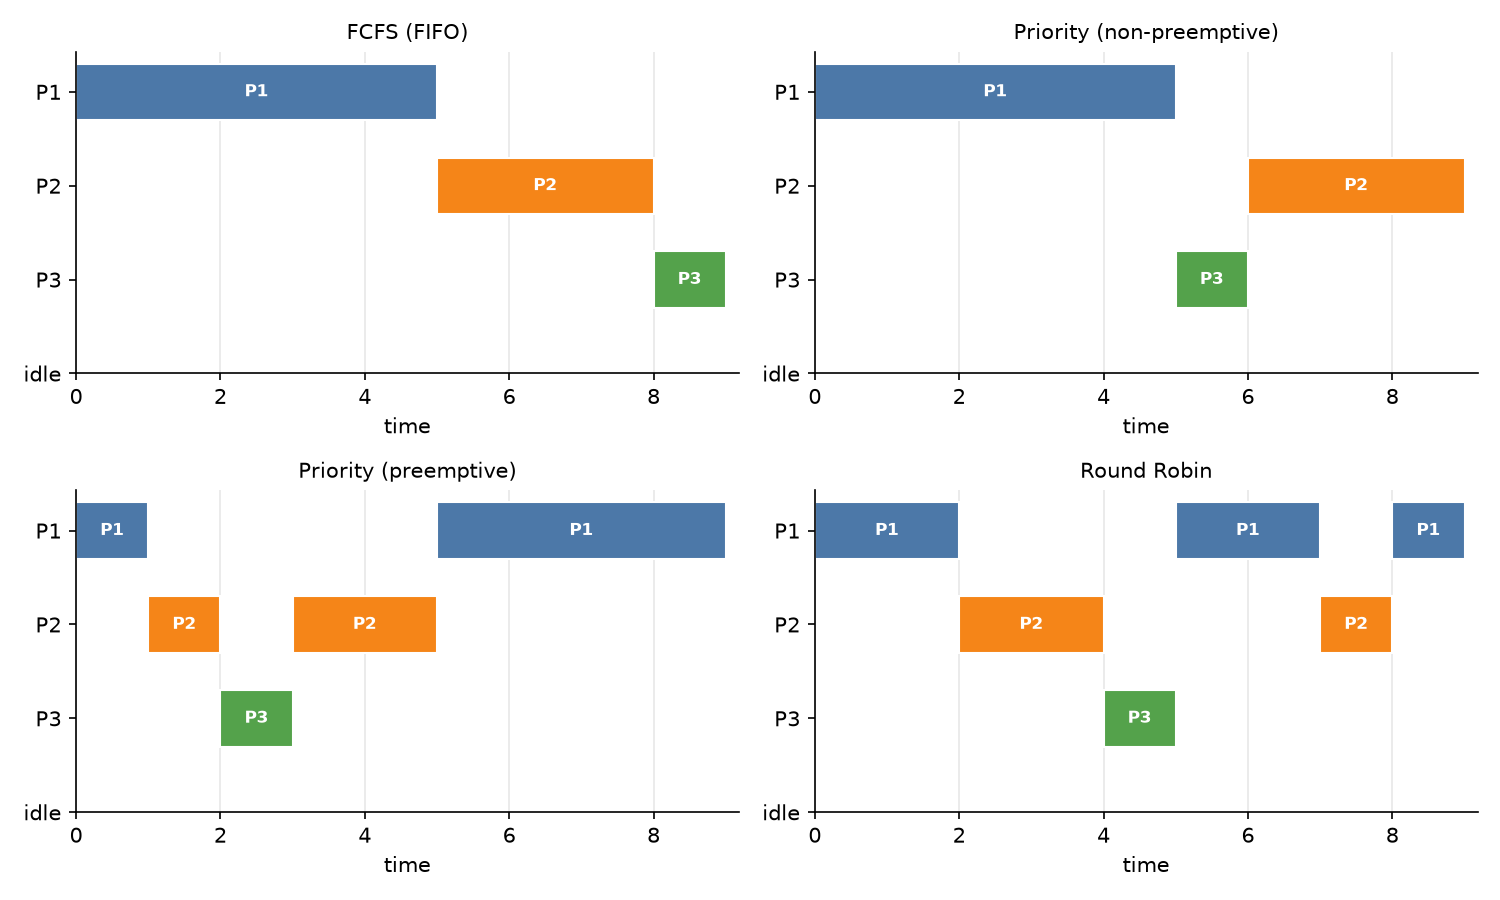
\includegraphics[width=\textwidth]{gantt_all.png}
    \end{column}
    \begin{column}{0.43\textwidth}
      We ran three jobs: one long, one medium and one short. Average times:\\[6pt]
      \begin{tabular}{lcc}
        \toprule
        Method & Waiting & Response \\
        \midrule
        FIFO & 3.33 & 3.33 \\
        Priority & 1.67 & 0.00 \\
        Round Robin & 3.33 & 1.00 \\
        \bottomrule
      \end{tabular}\\[6pt]
      \begin{itemize}
        \item Priority: least waiting
        \item Round Robin: quickest first reply
        \item Results match our hand calculation
      \end{itemize}
    \end{column}
  \end{columns}
\end{frame}

% ---------------------------------------------------------------
% 5. Working demo
\begin{frame}{Working demo}
  \begin{columns}[c]
    \begin{column}{0.48\textwidth}
      \textbf{What we will show}
      \begin{enumerate}
        \item See all running programs and pause or resume one
        \item See which program started which
        \item Watch live CPU and memory graphs
        \item Run the three methods and compare them
        \item Schedule real programs on this computer
      \end{enumerate}
    \end{column}
    \begin{column}{0.5\textwidth}
      \centering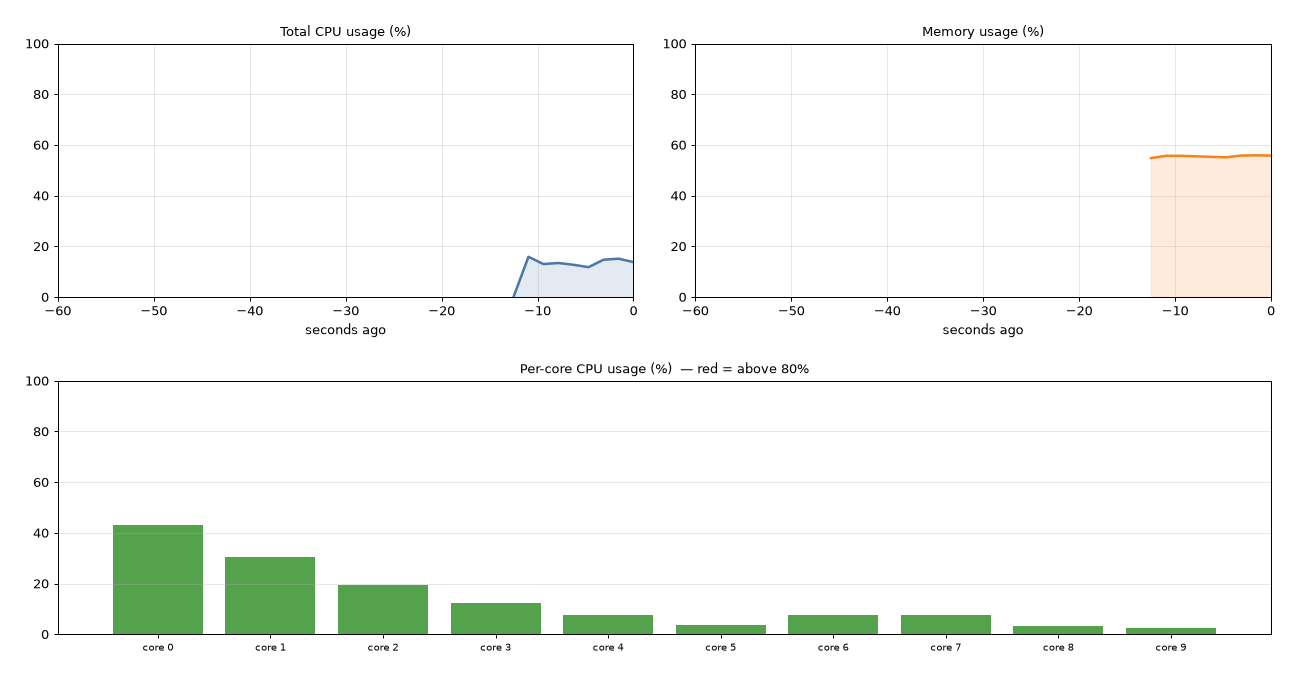
\includegraphics[width=0.85\textwidth]{system.png}\\[4pt]
      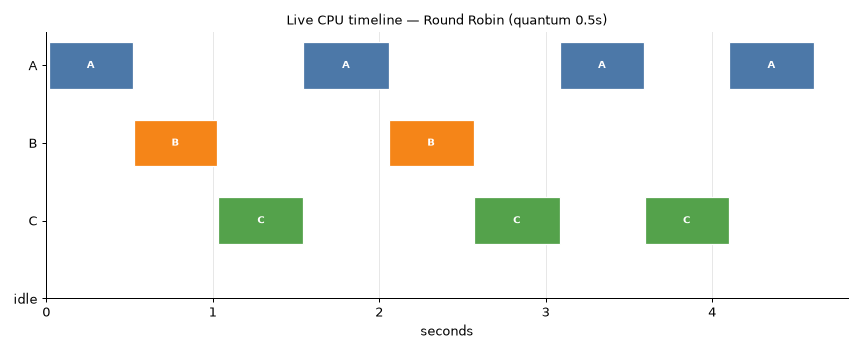
\includegraphics[width=0.85\textwidth]{real_rr.png}
    \end{column}
  \end{columns}
\end{frame}

% ---------------------------------------------------------------
% 6. Conclusion
\begin{frame}{Conclusion}
  \begin{itemize}
    \item One app shows \textbf{what is running now} and decides \textbf{who runs next}
    \item No single best method: Priority suits urgent jobs, Round Robin is the fairest
    \item Next: Shortest Job First
  \end{itemize}
  \vspace{1cm}
  \centering
  {\fontsize{40}{48}\selectfont\bfseries\color{structure} Thank you!}\\[0.4cm]
\end{frame}

\end{document}
